% CAPÍTULO 27 — «Mais fundo, mais junto» (andar 1: o que não se compra, o último pedaço)
% Fracasso que o abre: a queda conjunta mediu \numConjuntaExcesso{} vezes o que a independência
% prevê no corte de 5%, e o teto da proposição diz vinte --- o dado está a 36% do teto. Quem compra
% proteção no corte raso precisa do mesmo número no corte fundo, e as duas extrapolações que cabem
% no que já foi medido não concordam (a proporcional dá \numFundoPromessaProporcional; a gaussiana,
% \numFundoPromessaGaussiana). Este capítulo mede a TAXA com que a junta cai --- o expoente da cauda
% conjunta, lido direto do dado em cinco profundidades, com intervalo por bootstrap de blocos --- e
% o preço da extrapolação. Caderno: E38_mais_fundo (semente 105, posto \numFundoRhoPosto, ni por
% MLE \numFundoNi). Veredito: a razão cresce em todas as profundidades (\numFundoRazaoCinco a
% \numFundoRazaoUmQuarto) --- a junta cai mais devagar que a independência --- mas os intervalos dos
% expoentes SE SOREPÕEM (real \numFundoAlfaReal{} [\numFundoAlfaRealMin; \numFundoAlfaRealMax],
% gauss \numFundoAlfaGauss, t \numFundoAlfaT): a incerteza do expoente é ela mesma o resultado; e o
% preço mora na janela: a gaussiana da mesma janela cobre só \numFundoPrecoGaussJanela{} de
% \numFundoPrecoMedidos{} eventos fundos --- \numFundoPrecoDescoberto{} descobertos.
% Figuras: figuras/E38_mais_fundo_1.pdf (as taxas em log-log) e figuras/E38_mais_fundo_2.pdf (o
% preço no corte fundo, evento a evento).
% Costuras: o fecho do 26 entrega este capítulo como o quarto caso da compressão (a taxa); o fecho
% daqui carrega o parágrafo do enquadramento que vivia no 26; a nota de parte ganha o quinto nome.

\chapter{Mais fundo, mais junto}\label{cap:fundo}

\section{A pergunta que o corte raso não responde}

O capítulo da queda conjunta fechou com uma conta e um teto: as duas pernas rompem juntas
\numConjuntaExcesso{} vezes o que a independência prevê, no corte de cinco por cento --- e a
proposição do teto do par diz que naquele corte a conta não passa de vinte. O dado está a um terço
do teto. Mas quem compra a proteção no corte de cinco por cento precisa da mesma conta no corte de
meio por cento, e o livro não tinha esse número. As duas extrapolações que cabem no que já foi
medido não concordam: se a junta cai na taxa da própria margem, a razão no corte fundo vale
\numFundoPromessaProporcional; se cai na taxa da gaussiana com a correlação de posto do par, vale
\numFundoPromessaGaussiana. Não é a mesma proteção --- e a diferença entre as duas é o que este
capítulo mede.

\section{A profundidade como eixo}

O instrumento é o do capítulo da queda conjunta, sem peça nova: cada perna rompe o próprio corte de
janela e posto, e conta-se quantos dias as duas rombem contra o que a independência prevê. O que
muda é o eixo: o corte desce por cinco profundidades --- cinco, dois, um, meio e um quarto por cento
---, sempre na mesma janela de um ano e com o mesmo posto.

\begin{figure}[ht]
\centering
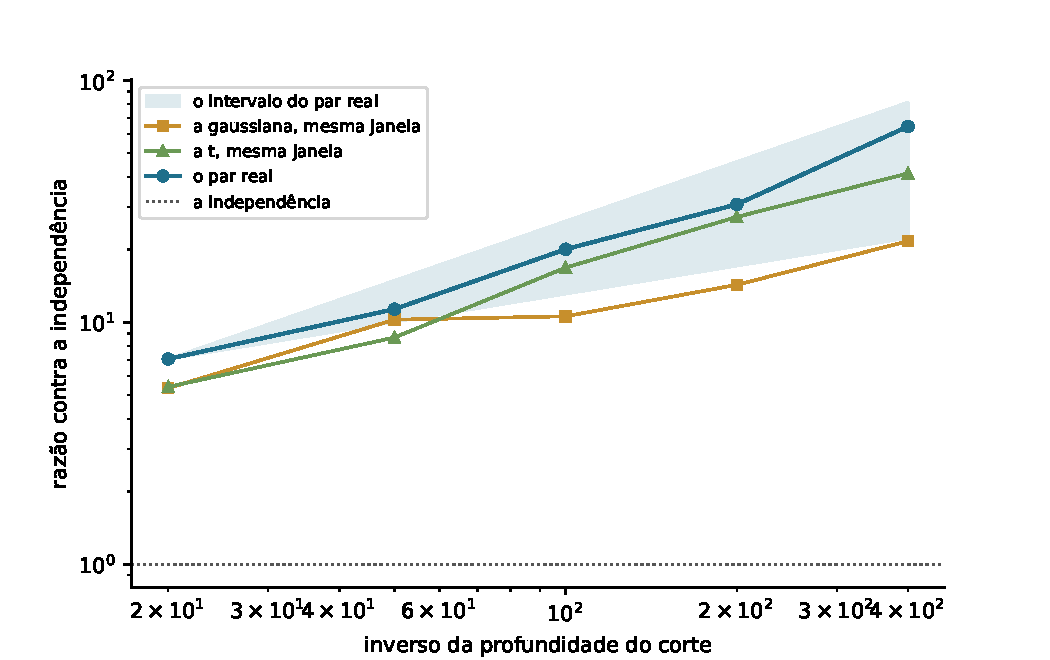
\includegraphics[width=\textwidth]{figuras/E38_mais_fundo_1.pdf}
\caption{A razão contra a independência em cada profundidade, em log-log --- a inclinação de cada
curva é a taxa com que a junta cai. O par real (azul, com a faixa do intervalo por bootstrap de
blocos) cresce de \numFundoRazaoCinco{} a \numFundoRazaoUmQuarto; a gaussiana da mesma janela
(laranja) cresce menos; a t (verde) acompanha o par de perto. A linha pontilhada é a independência,
que não cresce.}
\label{fig:fundo_taxas}
\end{figure}

A razão cresce em todas as profundidades: \numFundoRazaoCinco{} no corte de cinco por cento,
\numFundoRazaoDois{} no de dois, \numFundoRazaoUm{} no de um, \numFundoRazaoMeio{} no de meio,
\numFundoRazaoUmQuarto{} no de um quarto --- \numFundoJuntosCinco{} dias conjuntos no raso e
\numFundoJuntosUmQuarto{} no fundo, contra o esperado de \numFundoEsperadoCinco{} dias e de
\numFundoEsperadoUmQuarto. A resposta
à pergunta de abertura é medida: nem \numFundoPromessaProporcional, nem \numFundoPromessaGaussiana
--- \numFundoRazaoMeio. E a inclinação da reta em log-log --- o expoente da cauda conjunta --- vale
\numFundoAlfaReal, com intervalo de \numFundoAlfaRealMin{} a \numFundoAlfaRealMax{} no bootstrap de
blocos do capítulo do orçamento. Um expoente de \numFundoAlfaReal{} diz o seguinte: a probabilidade
conjunta cai quase na taxa da própria margem --- a junta quase não descola da margem quando o corte
afunda.

\section{O que o expoente não consegue separar}

Para que a diferença entre as estruturas fosse dependência e nada mais, os dois controles entram com
a MESMA correlação de posto do par, \numFundoRhoPosto --- a gaussiana com a lei da junta que a
assintótica anuncia \cite{savage1962mills,hashorva2003multivariate}, e a t com o grau de liberdade
escolhido por verossimilhança na grade declarada, \numFundoNi. Na mesma janela e com o mesmo
estimador: o expoente da gaussiana é \numFundoAlfaGauss, o da t é \numFundoAlfaT, o do par real é
\numFundoAlfaReal. Os três valores-para estão na ordem que a pedreira anunciava --- o par real junto
da t, a gaussiana acima ---, mas os intervalos se sobrepõem de ponta a ponta: de
\numFundoAlfaRealMin{} a \numFundoAlfaRealMax{} no real, de \numFundoAlfaGaussMin{} a
\numFundoAlfaGaussMax{} na gaussiana. Com esta amostra, o expoente não separa as estruturas --- e
essa é uma resposta, não um fracasso do desenho: a incerteza do expoente de cauda é ela mesma um
resultado \cite{taleb2020tail}. O controle negativo mostra de onde ela vem: pernas independentes dão
razão de um no corte raso, e no corte fundo um único dia extra muda a conta de ponta a ponta --- com
contagens de um dígito, o veredito não pode morar num ponto. Mora na monotonia: as cinco
profundidades do par real crescem todas, e nenhuma delas é um dia só.

\section{A pré-assíntota tem preço}

Havia uma terceira lição da pedreira, e ela também se mediu de novo: o expoente caminha com a janela
--- é a pré-assíntota, não instabilidade do dado \cite{taleb2018much}. A gaussiana da mesma janela
mede \numFundoAlfaGauss, contra o \numFundoAlfaAssintotico{} que a lei assintótica promete com este
posto; entre um e outro vai a diferença entre extrapolar a teoria e medir o mundo. É por isso que
toda comparação deste capítulo vive dentro da mesma janela e do mesmo estimador: fora dela, compara-se o
peixe com a isca.

\section{O preço, na moeda da proteção}

\begin{figure}[ht]
\centering
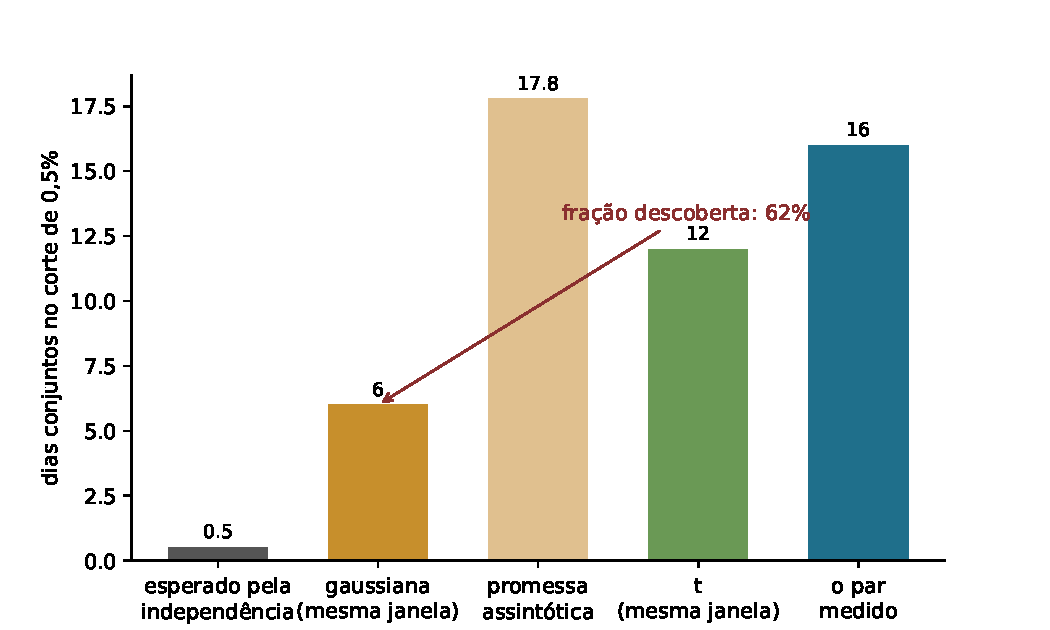
\includegraphics[width=\textwidth]{figuras/E38_mais_fundo_2.pdf}
\caption{Dias conjuntos no corte de meio por cento: o esperado pela independência, o que a
gaussiana da mesma janela entrega, o que a extrapolação assintótica promete, o que a t da mesma
janela entrega, e o medido no par. A seta marca a fração descoberta de quem dimensionou a proteção
pela gaussiana da janela.}
\label{fig:fundo_preco}
\end{figure}

Resta converter, e é a conversão que não existia entre a medida rasa e a conta funda. No corte de
meio por cento, o esperado pela independência é \numFundoPrecoEsperado{} de dia; a gaussiana da
mesma janela entrega \numFundoPrecoGaussJanela{} dias; a extrapolação assintótica promete
\numFundoPrecoAssintotico; a t da mesma janela, \numFundoPrecoTJanela; o par medido entrega
\numFundoPrecoMedidos. Quem dimensionou a proteção pela gaussiana da própria janela comprou
\numFundoPrecoDescoberto{} de buraco: de cada \numFundoPrecoMedidos{} dias conjuntos do corte fundo,
\numFundoPrecoGaussJanela{} estavam na conta. E a promessa assintótica, que quase cobre o medido, é
a que ninguém sabe que comprou --- porque o número impresso vinha do corte raso, e a taxa entre um e
outro nunca tinha sido medida.

\section{O que escapa da compressão, quarta vez}

O andar fecha a sua frase com cinco nomes: nenhum resumo devolve o que a compressão jogou fora ---
nem o mundo que não foi visto, nem o dia que foi apagado, nem o que a margem escondia, nem a taxa com que a
junta cai. Falta fechar pelo outro lado: o que não se compra tem preço mesmo assim, e é uma conta em
capital --- a última do andar.